\documentclass[a4paper,12pt]{article}
\usepackage[utf8]{inputenc}
\usepackage[italian]{babel}
\usepackage{hyperref}
\usepackage{graphicx}
\usepackage{longtable}
\usepackage{geometry}
\usepackage{booktabs}
\usepackage{listings}
\usepackage{caption}
\usepackage{float}
\geometry{margin=2.5cm}

\title{Honeypot}
\author{}
\date{}

\begin{document}

\maketitle

\tableofcontents
\newpage

\section{Introduzione} \label{1-introduzione}
Questo documento descrive l'architettura di rete utilizzata con Kathara per simulare un ambiente honeypot, consentendo l'analisi e lo studio di attacchi informatici in un contesto controllato. Il setup include vari dispositivi di rete e un server honeypot configurato per catturare e registrare le interazioni degli attaccanti.

\subsection{Kathara} \label{11-kathara}
Per il seguente lavoro, è stata utilizzata \href{https://www.kathara.org/}{Kathara}, una piattaforma di simulazione di rete che consente di creare e gestire scenari di rete complessi utilizzando container docker. Kathara è particolarmente utile per l'insegnamento e la sperimentazione in ambito networking.

\subsection{Immagini Docker} \label{12-immagini-docker}
Nel laboratorio sono state usate delle immagini Docker custom fornite da \href{https://hub.docker.com/u/theb0ys}{theb0ys}.

\begin{itemize}
    \item \href{https://hub.docker.com/r/theb0ys/base}{theb0ys/base}: Immagine base.
    \item \href{https://hub.docker.com/r/theb0ys/apache}{theb0ys/apache}: Server web Apache.
    \item \href{https://hub.docker.com/r/theb0ys/apache}{theb0ys/VERSIONE ALTERNATIVA}: Versione alternativa di Apache.
    \item \href{https://hub.docker.com/r/theb0ys/samba}{theb0ys/samba}: Condivisione file e stampanti.
    \item \href{https://hub.docker.com/r/theb0ys/mariadb}{theb0ys/mariadb}: DB MariaDB configurato per interfacce multiple.
\end{itemize}

\section{Topologia della rete} \label{2-topologia-della-rete}
\begin{figure}[H]
    \centering
    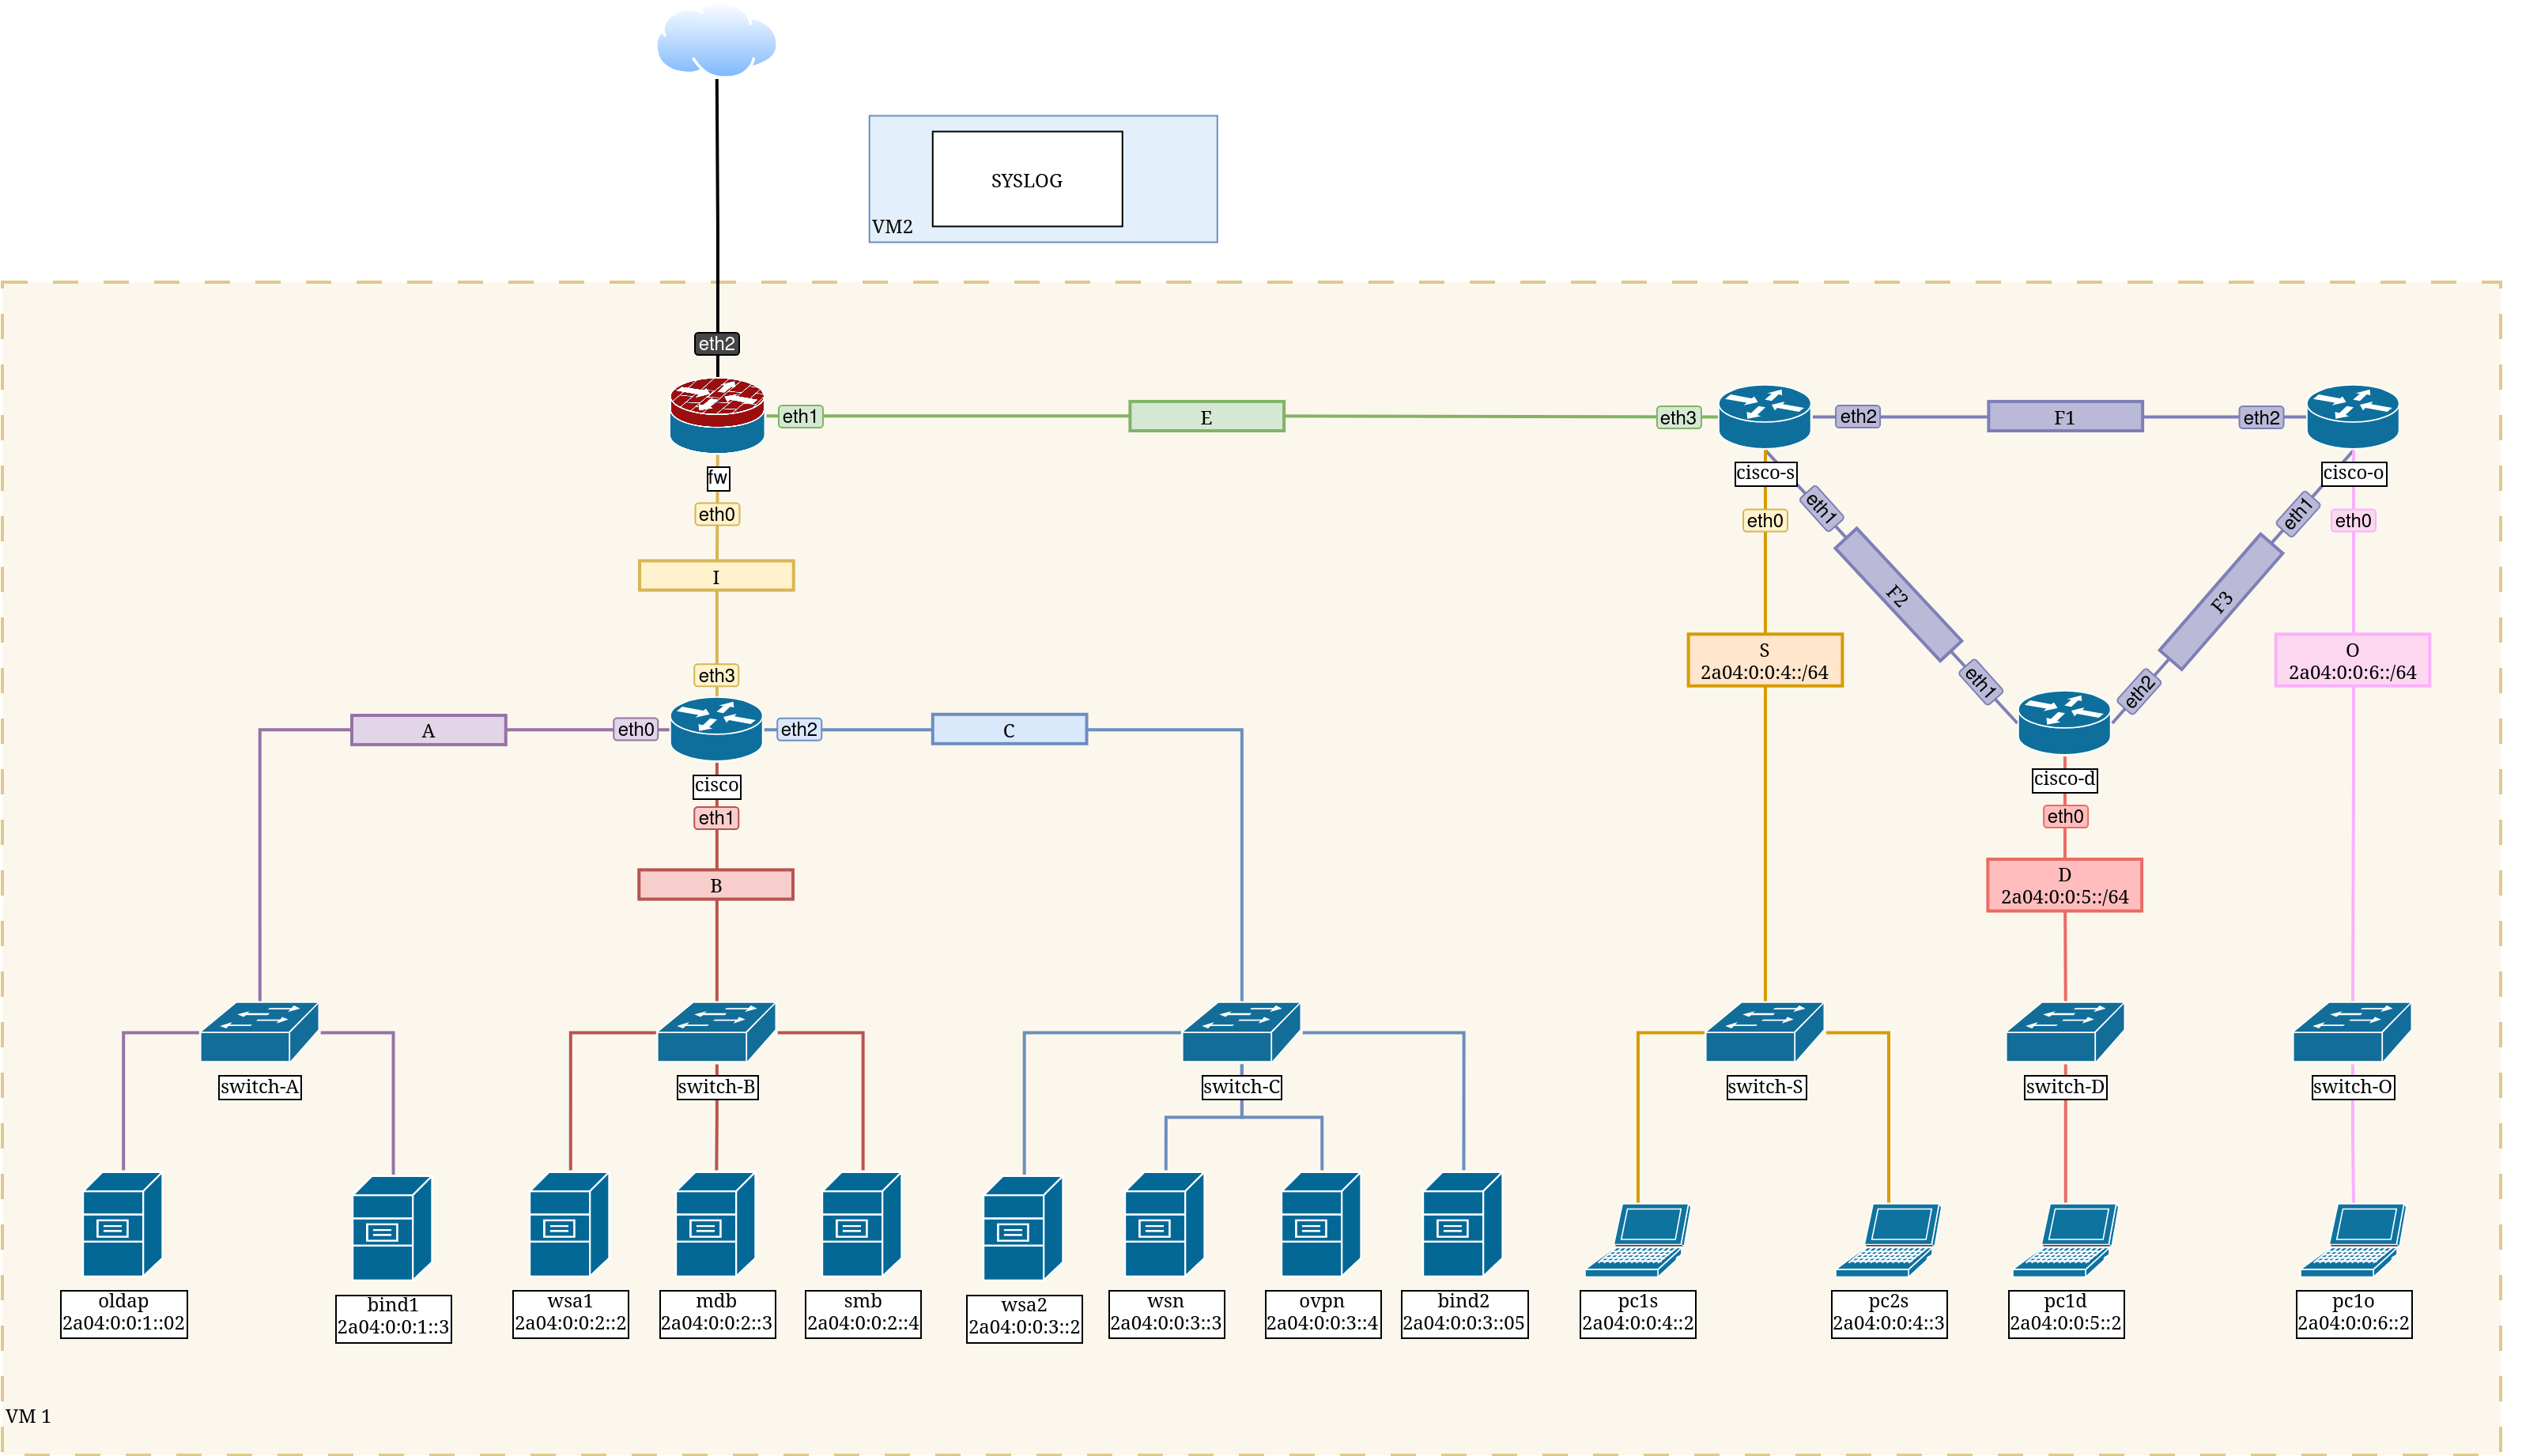
\includegraphics[width=0.8\textwidth]{img/network.drawio.png}
    \caption{Topologia della rete}
\end{figure}

\section{Spazio dei nomi} \label{3-spazio-dei-nomi}
\begin{figure}[H]
    \centering
    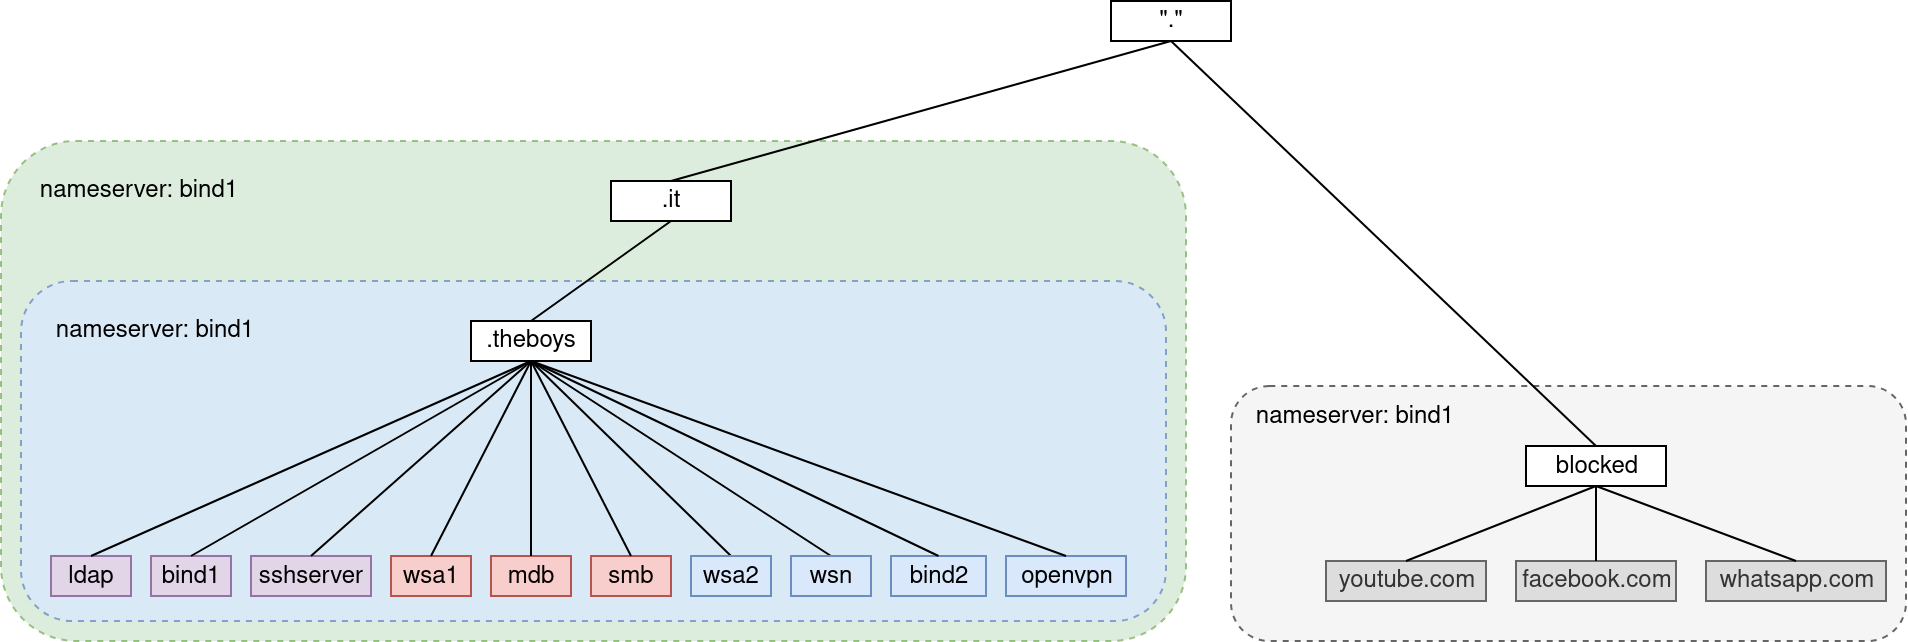
\includegraphics[width=0.8\textwidth]{img/namespace.drawio.png}
    \caption{Namespace}
\end{figure}

\section{Raggiungibilità} \label{4-raggiungibilità}
\begin{longtable}{lccccccc}
\toprule
DA/A & LAN A & LAN B & LAN C & LAN D & LAN O & LAN S & Internet \\
\midrule
bind1 & V & V & V & V & V & X & X \\
oldap &   &   &   &   &   & X & X \\
wsa1  & V & V & V & V & V & X & X \\
mdb   &   &   &   &   & X & X & V \\
wsa2  &   &   &   &   &   & X & V \\
nginx &   &   &   &   &   & X & V \\
openvpn & &  &  &  &  & X & V \\
bind2 & V & V & V & V & V & X & V \\
pcs1  & V & V & V & V & V & V & V \\
pcs2  & V & V & V & V & V & V & V \\
pcd1  &   &   &   &   &   & X & V \\
pco1  &   &   &   &   &   & X & V \\
\bottomrule
\end{longtable}

\section{LAN} \label{5-lan}
\subsection{LAN A} \label{51-lan-a}
\textbf{Descrizione}: La lan A è \dots \\
\textbf{Router}: \\
\textbf{Hosts}:
\begin{itemize}
    \item ldap
    \item bind1: DNS server bind9, risoluzione per la intranet.
\end{itemize}

\subsection{LAN B} \label{52-lan-b}
\textbf{Descrizione}: La lan B è \dots \\
\textbf{Hosts}:
\begin{itemize}
    \item wsa1: Web server Apache2 interno.
    \item mdb
    \item smb
\end{itemize}

\subsection{LAN C} \label{53-lan-c}
\textbf{Descrizione}: La lan C è \dots \\
\textbf{Hosts}:
\begin{itemize}
    \item wsa2: Web server Apache2 con WP + MariaDB.
    \item wsn: Web server nginx per Internet.
    \item openvpn
    \item bind1
\end{itemize}

\subsection{LAN S} \label{54-lan-s}
\textbf{Descrizione}: La lan S è \dots \\

\subsection{LAN D} \label{55-lan-d}
\textbf{Descrizione}: La lan D è \dots \\

\subsection{LAN O} \label{56-lan-o}
\textbf{Descrizione}: La lan O è \dots \\

\section{NAT}
\subsection*{Chain PREROUTING (nat) – Port Forwarding}
\begin{longtable}{ccccccccccc}
\toprule
\# & target & prot & in & out & source & dest & src port & dst port & DNAT to & Note \\
\midrule
1 & DNAT & tcp & eth4 & & 0.0.0.0/0 & 0.0.0.0/0 & any & 22 & 192.168.0.4:22 & sshserver \\
2 & DNAT & tcp & eth4 & & 0.0.0.0/0 & 0.0.0.0/0 & any & 80 & 192.169.0.2:80 & ws1a \\
3 & DNAT & tcp & eth4 & & 0.0.0.0/0 & 0.0.0.0/0 & any & 139 & 192.169.0.4:139 & smb \\
4 & DNAT & tcp & eth4 & & 0.0.0.0/0 & 0.0.0.0/0 & any & 445 & 192.169.0.4:445 & smb \\
5 & DNAT & tcp & eth4 & & 0.0.0.0/0 & 0.0.0.0/0 & any & 8080 & 192.170.0.3:80 & wsn \\
\bottomrule
\end{longtable}

\subsection*{Chain FORWARD – Allow NAT Traffic}
\begin{longtable}{ccccccccccc}
\toprule
\# & target & prot & in & out & source & dest & src port & dst port & Note \\
\midrule
1 & ACCEPT & tcp & & & 0.0.0.0/0 & 192.168.0.4 & any & 22 & sshserver \\
2 & ACCEPT & tcp & & & 0.0.0.0/0 & 192.169.0.2 & any & 80 & ws1a \\
3 & ACCEPT & tcp & & & 0.0.0.0/0 & 192.169.0.4 & any & 139 & smb \\
4 & ACCEPT & tcp & & & 0.0.0.0/0 & 192.169.0.4 & any & 445 & smb \\
5 & ACCEPT & tcp & & & 0.0.0.0/0 & 192.170.0.3 & any & 80 & wsn \\
\bottomrule
\end{longtable}

\section{Firewall} \label{6-firewall}

\subsection*{Chain INPUT (Policy ACCEPT)}
(Nessuna regola specificata)

\subsection*{Chain FORWARD (Policy DROP)}
\begin{longtable}{cccccccccc}
\toprule
\# & target & prot & in & out & source & dest & src port & dst port \\
\midrule
2 & ACCEPT & all & & & 192.168.0.0/24 & & & \\
3 & ACCEPT & all & & & 192.169.0.0/24 & & & \\
4 & ACCEPT & all & & & 192.170.0.0/24 & & & \\
5 & ACCEPT & tcp & & & 192.168.1.0/24 & & & 22 \\
6 & ACCEPT & all & & & & & & \\
\bottomrule
\end{longtable}

\subsection*{Chain OUTPUT (Policy ACCEPT)}
(Nessuna regola specificata)

\section{Accounts} \label{7-accounts}

\subsection*{SSH}
\begin{longtable}{lll l}
\toprule
Host & Username & Password & Tipo di Account \\
\midrule
bind & senior & 1Password! & Amministratore Senior \\
bind & junior & 2Password! & Amministratore Junior \\
ldap & senior & 1Password! & Amministratore Senior \\
mdb & senior & 1Password! & Amministratore Senior \\
openvpn & senior & 1Password! & Amministratore Senior \\
smb & senior & 1Password! & Amministratore Senior \\
wsa1 & senior & 1Password! & Amministratore Senior \\
wsa1 & junior & 2Password! & Amministratore Junior \\
wsa2 & senior & 1Password! & Amministratore Senior \\
wsa2 & junior & 2Password! & Amministratore Junior \\
wsn & senior & 1Password! & Amministratore Senior \\
wsn & junior & 2Password! & Amministratore Junior \\
\bottomrule
\end{longtable}

\subsection*{Samba}
\begin{longtable}{lll l}
\toprule
Host & Username & Password & Tipo di Account \\
\midrule
smb & mario & 1as-aoi & Dirigente \\
smb & filippo & lolw-9u! & Dipendente \\
\bottomrule
\end{longtable}

\subsection*{DB / phpMyAdmin}
\begin{longtable}{lll l}
\toprule
Host & Username & Password & Tipo di Account \\
\midrule
mdb & senior & 1Password! & Amministratore Senior \\
mdb & junior & 2Password! & Amministratore Junior \\
mdb & pluto & pluto & Da eliminare - funziona solo in v0.5-ufficiale in su \\
\bottomrule
\end{longtable}

\end{document}
